\documentclass[12pt]{article}

\usepackage[margin=0.8 in]{geometry}
\usepackage{amsmath}
\usepackage{amssymb}
\usepackage{mathtools}
\usepackage{enumerate}
\usepackage{verbatim}
\usepackage{amsthm}
\usepackage{hyperref}

\title{}
%\content{}



\let \proj \undefined
\newcommand{\p}{\partial}
\newcommand{\R}{ \mathbb{R}}

\DeclareMathOperator{\proj}{proj}
\newcommand{\sS}{\mathscr{S}}
\DeclareMathOperator{\comp}{comp}
\newcommand{\A}{\mathcal{A}}
\newcommand{\D}{\mathcal{D}}
\newcommand{\e}{\epsilon}
\newcommand{\et}{\tilde{\e}}
\newcommand{\vr}{\vec{r}{}}
\newcommand{\vF}{\vec{F}}
\newcommand{\triple}{\iiint_E f(x,y,z)dV}
\renewcommand{\lg}{\langle}
\newcommand{\rg}{\rangle}
\newcommand{\Q}{\frac{\p Q}{\p x}}
\renewcommand{\P}{\frac{\p P}{\p y}}
\let\implies\Rightarrow
\newcommand{\n}{\nabla}
\newcommand{\Fline}{\vF\cdot d\vr}
\newcommand{\vi}{\vec{i}}
\newcommand{\vj}{\vec{j}}
\newcommand{\vk}{\vec{k}}
\DeclareMathOperator{\curl}{curl}
\newcommand{\vn}{\vec{n}}
\newcommand{\vS}{\vec{S}}
\newcommand{\flux}{\iint_S \vF\cdot d\vS}
\newcommand{\vG}{\vec{G}}
\let \div \undefined
\DeclareMathOperator{\div}{div}


\newcommand{\rcross}{\vr_u\times\vr_v} 




\newenvironment{solution}
  {\begin{proof}[Solution]}
  {\end{proof}
  
  }
\newtheorem{example}{Example}
\newtheorem{exercise}{Exercise}
\newtheorem{theorem}{Theorem}
\newtheorem{defn}{Definition}


\begin{document}
\section*{Stokes' Theorem}
What to know:
\begin{enumerate}
\item Be able to state Green's Theorem
\item Be able to use Green's Theorem to compute line integrals.
\end{enumerate}




In this section we will generalize Green's theorem to surfaces in $\R^3$. Let's start with a definition. 
\begin{defn}
Suppose $S$ is an oriented surface with unit normal vector field $\vn$ the boundary of which is the curve $c$. We say that $c$ is \textbf{positively oriented} if the direction it is transversed and $\vn$ follow the right hand rule. That is, when the four fingers of your right hand other than the thumb are following the curve, your thumb should be pointing in the direction of $\vn$. If this is not the case, we say that $c$ is \textbf{negatively oriented}.
\end{defn}




\begin{figure}[h]
\centering
\parbox{5cm}{
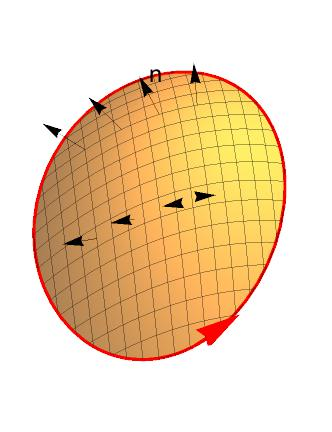
\includegraphics[scale=.4]{right.jpeg}
\caption{Positive orientation}
\label{}}
\qquad
\begin{minipage}{5cm}
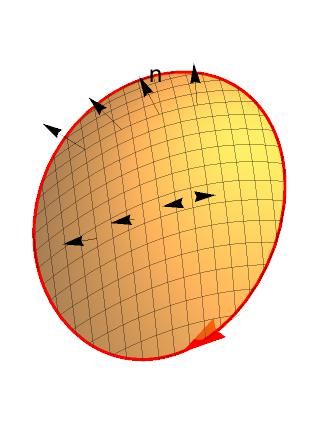
\includegraphics[scale=.4]{negative.jpeg}
\caption{Negative oriantation}
\label{fig:2figsB}
\end{minipage}
\end{figure}




\begin{itemize}
\item If our surface lies on the $xy$ plane and we give it the orientation determined by the the vector field $\lg 0,0,1\rg$, the boundary curve being positively oriented is the same as saying that it is oriented counterclockwise.
\item Another way you could think of positive orientation is that  if you're walking on the curve with your head towards the direction of $\vn$, the surface should be on your left.
\item A cat explaining the right hand rule, \href{http://sites.math.washington.edu/~neptamin/324Au17/Notes/16.8/righthandrule.gif}{here}.
\end{itemize}


Now recall that in the previous section we saw the following example: 
\begin{example}
Let $S$ be the upper hemisphere of the unit sphere oriented \textbf{downwards}, and let $\vF=\lg -y,x,1\rg.$ Compute the flux of $\curl\vF $ across $S$.
\end{example}
The answer we found was $\iint_S\curl \vF\cdot d\vS=-2\pi$. Now let's do the following:
\begin{exercise}
Compute the line integral $\int_c\vF\cdot d\vr$, where $c$ is the clockwise parametrized unit circle on the $xy$ plane, that is, $$c(t)=\left (\cos(-t),\sin(-t),0\right ).$$
\end{exercise}
You should find $-2\pi$. Observe that $c$ is the positively oriented boundary curve of the unit upper hemisphere centered at the origin with downward orientation, as we can see from the picture \ref{fig3}. 

\begin{figure}[h]
\begin{center}
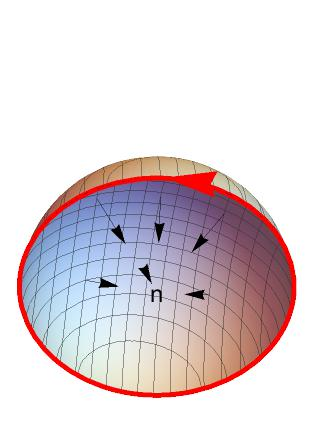
\includegraphics[scale=.4]{hemi.jpeg}
\caption{The hemisphere with downward orientation and its boundary, viewed from below.}
\label{fig3}
\end{center}
\end{figure}


The fact that we find $$\iint_S\curl \vF\cdot d\vS=\int_c \vF\cdot d\vr$$ is not a coincidence, and it is a consequence of the following theorem:


\begin{theorem}
(Stokes) Let $S$ be an oriented parametric surface with its boundary consisting of a curve $c$, that is assumed to have positive orientation, and let be and $\vF$ be a vector field in $\R^3$ with differentiable coefficients. Then $$\iint_S\curl \vF\cdot d\vS=\int_c \vF\cdot d\vr.$$ 
\end{theorem}



\textbf{Remarks:} 
\begin{enumerate}
\item If the orientation of $c$ is negative, $-c$ is positively oriented, and therefore
$$\iint_S\curl \vF\cdot d\vS=\int_{-c} \vF\cdot d\vr=-\int_{c} \vF\cdot d\vr.$$

\item We often denote the positively oriented boundary curve of $S$ by $\p S$, so Stokes' theorem becomes  $$\iint_S\curl \vF\cdot d\vS=\int_{\p S} \vF\cdot d\vr.$$ 


\item Why is Stokes' Theorem useful? In our context, it becomes most useful when we have to compute a line integral over a curve that can be conveniently written as the boundary of a surface. In this sense, it works in a way completely analogous to Green's Theorem, except for more general surfaces in $\R^3$. In Real Life, it is particularly useful for computing line integrals over closed curves that consist of several distinct smooth segments that would require you to write a sum of several integrals.

In general, Stokes' theorem isn't very useful for computing the surface integral of a vector field $\vG$, unless it is already known that the vector field $\vG$ can be written as $\vG=\curl\vF$ for another vector field $\vF$. However, we already saw that this can't happen unless $\div{\vG}\equiv 0$ and this condition is quite restrictive: Most vector fields can't be written as the curl of another vector field.





\item Stokes' Theorem generalizes Green's Theorem in the following sense: Let $D$ be a domain in $\R^2$, $c=(x(t),y(t))$ be its boundary curve with counterclockwise orientation and $\vF(x,y)=\lg P(x,y),Q(x,y)\rg$ be a vector field in $\R^2$. We embed $D$ to a surface $S$ in $\R^3$ using the parametrization $$\vr(u,v)=\lg u,v,0\rg,(u,v)\in D$$ band we give it upward orientation, that is given by the constant unit normal vector field $\vn=\lg 0,0,1\rg$. We finally extend $\vF$ as a vector field in $\R^3$ by setting $$\vF(x,y,z)=\lg P(x,y),Q(x,y),0\rg.$$

We find $$\curl \vF=\lg 0,0, \Q-\P\rg.$$

Now we apply Stokes' Theorem on $S$ and find $$\int_c \vF \cdot d\vr=\iint_S\curl\vF\cdot d\vS=\iint_D\lg 0,0, \Q-\P\rg\cdot \lg 0,0,1\rg dA=\iint_D \Q-\P dA,$$
which is Green's Theorem.


\item ``Independence of surface'': Suppose that we have two oriented surfaces $S_1$ and $S_2$ that share the same positively oriented boundary $c$. For example, $S_1$ could be the lower hemisphere of the unit sphere and $S_2$ the upper hemisphere of the unit sphere, both with upward orientation so that their common boundary is the positively oriented unit circle on the $xy$ plane. Then $$\iint_{S_1}\curl\vF\cdot d \vS=\int_c\Fline =\iint_{S_2}\curl\vF\cdot d \vS.$$

Observe the analogy with the FTC, where we had independence of path for a vector field that was the ``derivative'' of a scalar function. Here we have ``independence of surface'' for a vector field $\vec{G}$ assuming it is the ``derivative'' of another vector field: It can be written as $\vec{G} =\curl\vF$. As remarked already, this can't be the case for vector fields $\vec{G}$ that don't satisfy $\div \vec{G}\equiv 0$.

This also means that when we want to compute a line integral along a closed curve, then we are free to choose \textbf{any} surface that has our curve as its boundary.


\item For any closed surface $S$, $\iint_S\curl\vF\cdot d\vS=0$. Can you prove this using Stokes' Theorem?



\item What is Stokes' Theorem saying from a physical point of view? When we defined the $\curl $ operator, there was a comment about its relation to rotations. We mentioned that $\curl\vF$ at a point $p$ corresponds to the work produced by the vector field when an infinitesimally small circulation is happening near the point, on the plane perpendicular to the direction of $\curl\vF(p)$. Then, Stokes' Theorem tells us that those amounts of work produced by the field on infinitesimally small circulations on the points of a surface add up the work produced while a large circulation is happening, on the boundary of the surface (look at picture \ref{figr}). 
\begin{figure}[h]
\begin{center}
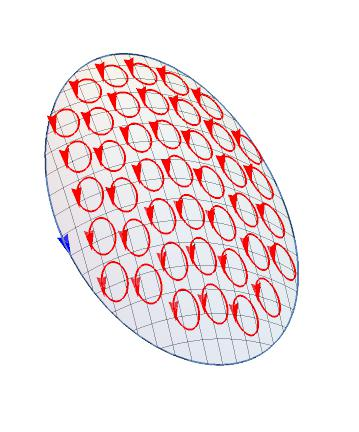
\includegraphics[scale=.6]{circulation.jpeg}
\caption{``Summing up microscopic circulations leads to a macroscopic circulation''}
\label{figr}
\end{center}
\end{figure}


\end{enumerate}







\end{document}

